%---------------------------------------------------------------------------
% Monitoring Hub component.
%
%---------------------------------------------------------------------------


\section{Monitoring Hub}
\label{sec:arch_monitoring_hub}


Monitoring Hub is the core component of system. If using layered model to analyze application, Monitoring Hub should be
treated as logic layer - placed between presentation layer (GUI) and data access layer (transport proxies). It
provides services to GUI, and uses Transport Proxies with Knowledge components.
It main responsibilities include resources management (registering new resources, discovery dependent resources),
measurements management (creation, pausing, resuming and termination) and creation of scheduled jobs that pools for
capability values and pushes new values to registered listeners. 

When user wants to start monitoring new resource, he or she must choose which Monitoring Hub will be used for this
task. This decision, creates direct association between chosen Hub, resource to monitor and all it's
child resources discovered during registration. This association constraints, that all further request calls in
context of given resource will be processed by Monitoring Hub associated during registration or discovery process.

To make high level components loosely coupled, Monitoring Hub isn't aware of details about other components. To be able
to provide it's services it uses transport proxies and knowledge components, but it interacts with them only using
commonly known interfaces. Additionally it isn't aware about existence of GUI components at all - it just provides
services by implementing given interface, and to be able to notify about variety of events, it uses also common listener
interfaces.

\subsection{Decomposition of Monitoring Hub}

\begin{figure}[h]
  \centering
  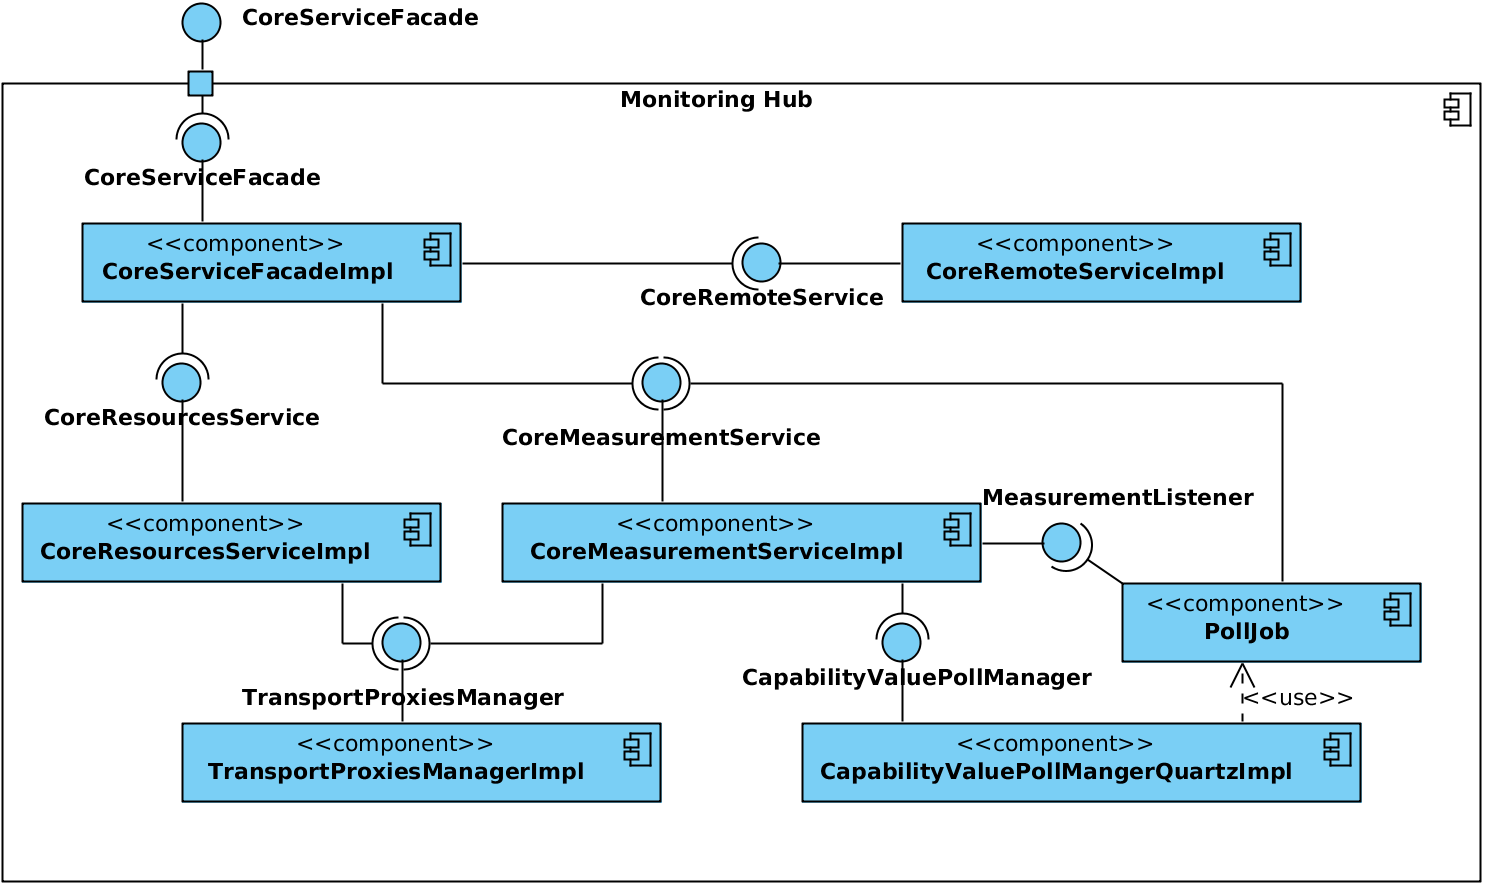
\includegraphics[width=0.9\textwidth]{decomposition_mon_hub}
  \caption{Communication diagram - adding of new resource}
  \label{fig:decomposition_mon_hub}
\end{figure}

Further decomposition of application, the internal details of Monitoring Hub can be found
in Figure~\ref{fig:decomposition_mon_hub}. In this component, author have distinguished following low level components:

\begin{itemize}

 \item {\bf CoreServiceFacadeImpl}~~~~~~~~~~~~~~~~~~~~~~~~~~~~~~~~~~~~~~~~~~~~~~~~~~~~~~~~\linebreak
Facade that allows access to all Monitoring Hub functionalities from single interface (CoreServiceFacade, shared with
GUI and Monitoring Hub Application high level components). This wrapper is needed to ease remote access - exposing
and using one interface with any remoting middleware is easier than multiple ones. Having multiple interfaces in most
cases would require multiple socket connections which can be source of additional problems. We should tend to use as
small amount connections as possible, because more connections are being used, than system becomes more and more prone
to network configuration issues (e.g. firewalls).
Additionally, using single facade improves code style, as with facade, only one interface has to be visible for all
other components that are its clients.

 \item {\bf CoreRemoteServiceImpl}~~~~~~~~~~~~~~~~~~~~~~~~~~~~~~~~~~~~~~~~~~~~~~~~~~~~~~~~\linebreak
Service responsible for processing requests related to remote management of Monitoring Hub. It has two main
responsibilities: it allows to register remote listening interfaces and it dispatches local events (new resource,
new capability value etc.) to remote listeners in aggregated manner. Distributed dispatch of events requires a bit
different approach than local one (local one, means dispatch inside of single JVM process). First of all, in most cases
remote interface that will receive notifications in most cases uses different signature, to allow handling exceptions
related to networking. Additionally, to reduce amount of remote calls and thus improve efficiency,
CoreRemoteServiceImpl aggregates events into batches and notifies remote listeners using a generated package of
events. Such an approach doesn't pollute measuring results, because each measurement value has associated gather
timestamp (see~\ref{subsec:arch_comm_protocol}), initialized by component that grabs given value, at the exact moment,
of measurement.
Additionally, as events related to resources addition/removal doesn't require such a strict time association, those
events can be aggregated without any issues.

 \item {\bf CoreResourcesServiceImpl}~~~~~~~~~~~~~~~~~~~~~~~~~~~~~~~~~~~~~~~~~~~~~~~~~~~~~~~~\linebreak
Service responsible for resources management - registering new ones, discovery of their children, and getting all
registered and discovered. It's also used to get more details about resource, like capabilities that given resource may
have.


 \item {\bf CoreMeasurementServiceImpl}~~~~~~~~~~~~~~~~~~~~~~~~~~~~~~~~~~~~~~~~~~~~~~~~~~~~~~~~\linebreak
Measurement services - can be used to create, pause, stop or terminate a measurement. Additional it gather current
values of capabilities. It's used by PollJob for that purpose. It implements MeasurementListener interface to be able
to receive notification about new capability values polled by PollJob. 

 \item {\bf TransportProxiesManagerImpl}~~~~~~~~~~~~~~~~~~~~~~~~~~~~~~~~~~~~~~~~~~~~~~~~~~~~~~~~\linebreak
Manages registered transport proxies. It is used by other components to get all transport proxies or to lookup transport
proxy that can be used to manage given resource.

 \item {\bf CapabilityValuePollManagerImpl}~~~~~~~~~~~~~~~~~~~~~~~~~~~~~~~~~~~~~~~~~~~~~~~~~~~~~~~~\linebreak
Is responsible for scheduling polling jobs needed to run measurement.

 \item {\bf PollJob}~~~~~~~~~~~~~~~~~~~~~~~~~~~~~~~~~~~~~~~~~~~~~~~~~~~~~~~~\linebreak
Job triggered with configured interval. It simply polls for current capability value and push it to listeners specified
during creation.

\end{itemize}

\pagebreak

\subsection{Most important data flows}

This section contains description of most important data flows inside Monitoring Hub component. It covers actions
of adding new resources, adding new measurements and dispatching new capability value notification.

Figure~\ref{fig:comm_mh_add_res} depicts communication diagram of adding new resources. In this scenario, external GUI
components initiates action - first step is request registerResource send by it to CoreServiceFacadeImpl. Facade simply
delegates this call to CoreResourcesServiceImpl, which will perform actual registration.
In next step, CoreResourcesServiceImpl tries to find proxy capable to communicate with given resource. To achieve that
it calls TransportProxiesManagerImpl. What should be noticed, Transport Proxy is an external component to
Monitoring Hub. After successfully obtaining transport proxy, CoreResourcesServiceImpl performs call on it to
register given resource. If this registration succeeds, resources service uses another external component, Knowledge, to
get all types of child resources that resource in subject may have. Using this list, service requests TransportProxy to
discover all children of resource being registered. After successful discovery, notification containing resources is
being dispatched to all listeners either directly, when given Monitoring Hub is embedded into GUI, or using
CoreRemoteServiceImpl to dispatch to all remote GUI components registered.

\begin{figure}[h]
  \centering
  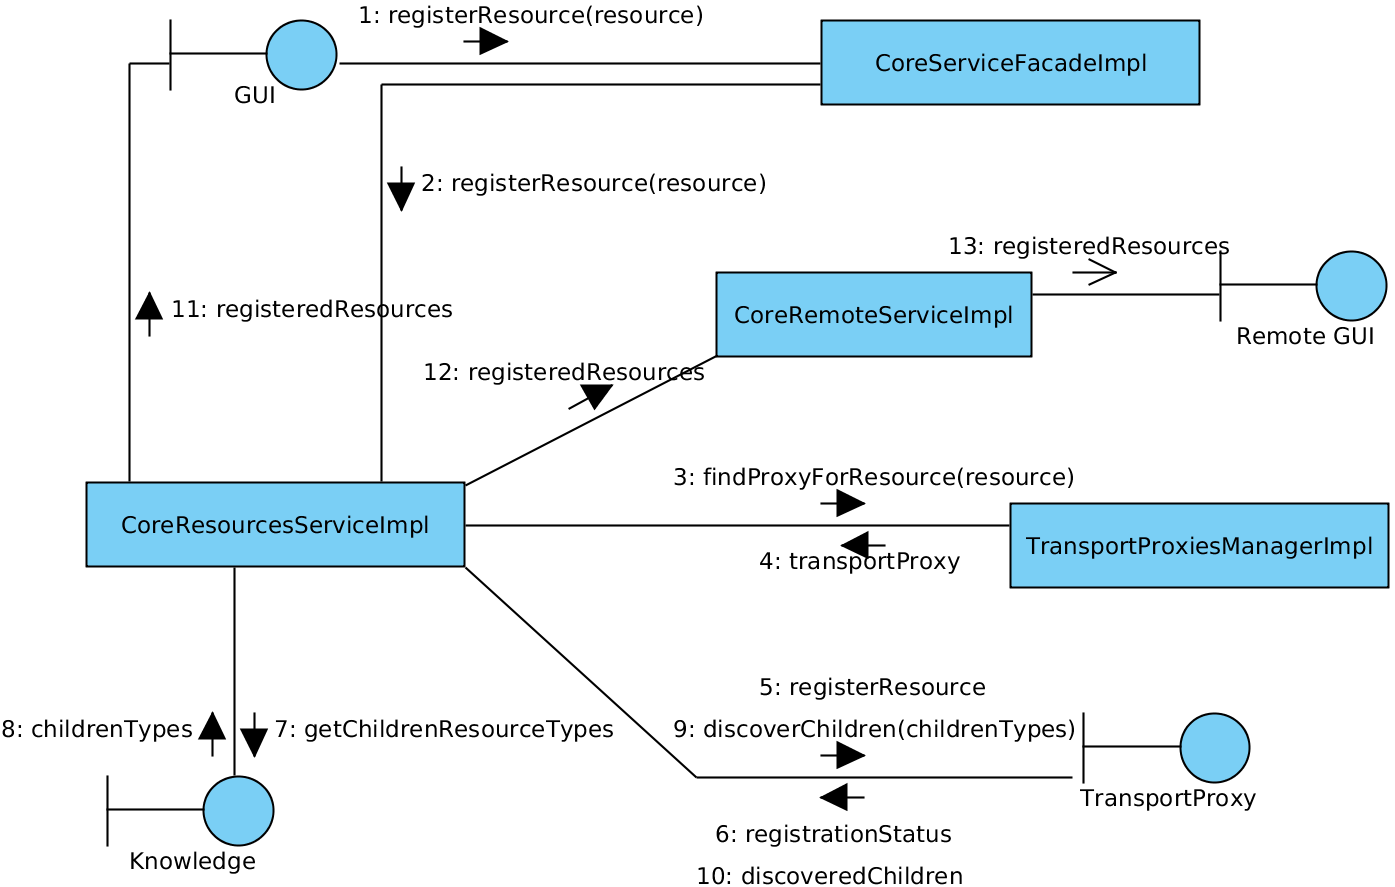
\includegraphics[width=0.9\textwidth]{comm_mh_add_res}
  \caption{Monitoring Hub Communication diagram - adding new resource}
  \label{fig:comm_mh_add_res}
\end{figure}



Communication diagram covering action of addition new measurement can be found in
Figure~\ref{fig:comm_mh_add_measurement}. In this scenario, again GUI component is initiator. First request is
sent to CoreServiceFacadeImpl, GUI component calls method getResourceCapabilities. It will use those capabilities to
show the user UI compnent, which will let him choose which capability to measure. Facade delegates query to
CoreResourcesServiceImpl, which passes it to external Knowledge component. Resulting list of capability URI's is being
passed all way back, to the GUI component. Next, user selects which capability should be measured. On selection event,
GUI requests CoreServiceFacadeImpl to create measurement using given definition (see Table~\ref{tab:TO_MeasurementDef}).
Request is delegated to CoreMeasurementServiceImpl which is responsible for actual creation of measurement. Measurement
service requests CapabilityValuePollManagerImpl to create new instance of PollJob class. After creating polling job,
measurement service generates measurement id, stores it internally with measurement definition, and returns it to
requester. This identifier is then passed back to GUI, which will use it in any future call referring newly created
measurement toto use itso this component can use it to reference incoming CapabilityValues and to be able to update or
remove measurement.

\begin{figure}[h]
  \centering
  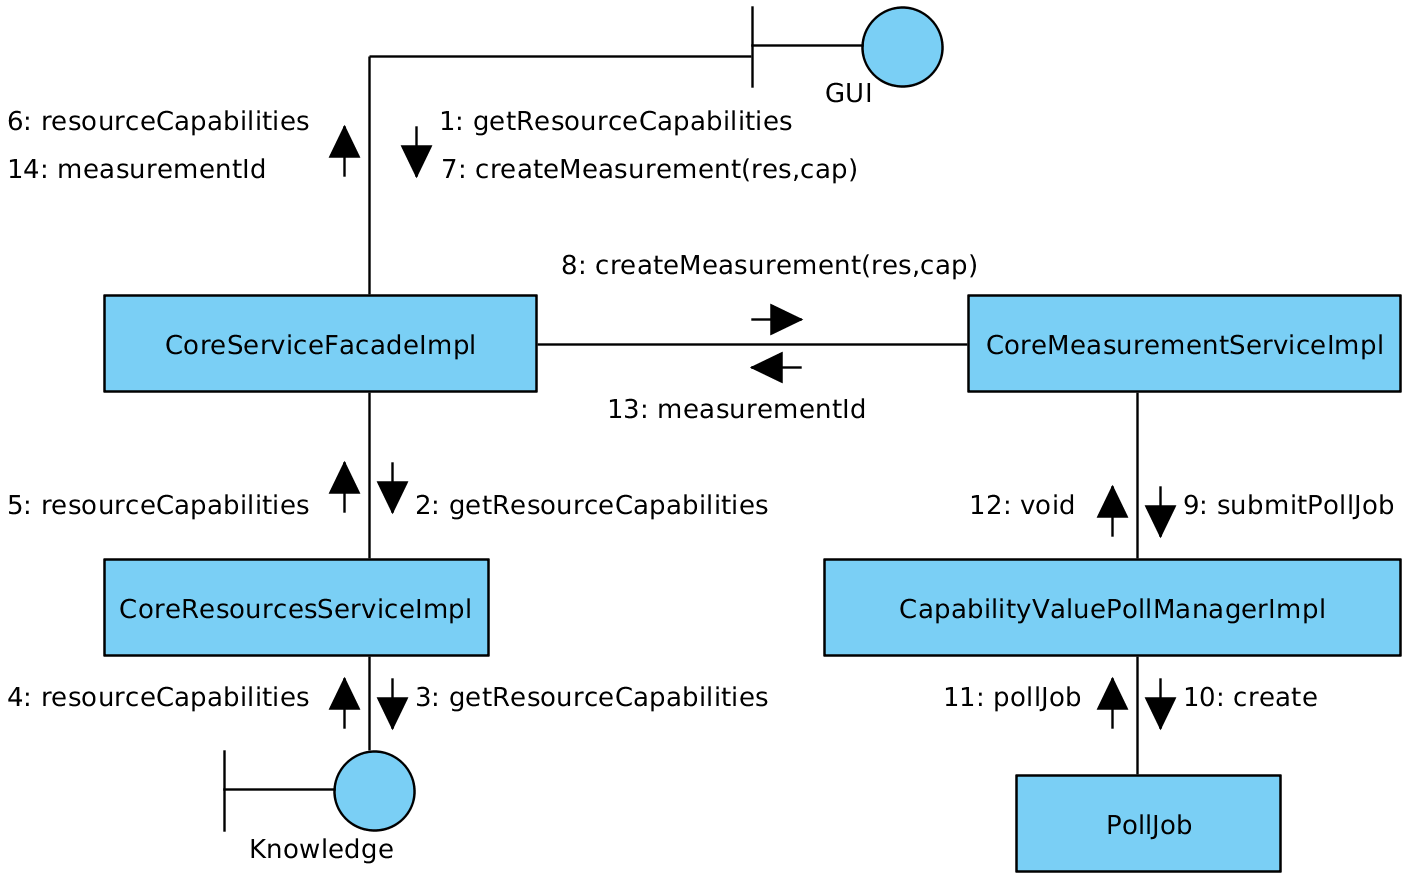
\includegraphics[width=0.8\textwidth]{comm_mh_add_measurement}
  \caption{Monitoring Hub Communication diagram - adding new measurement}
  \label{fig:comm_mh_add_measurement}
\end{figure}

Last data flow covered in this section describes gathering and publishing capability values. Action is initialized by
CapabilityValuePollManagerImpl. It's internal scheduler triggers previously created PollJob which contains measurement
definition (URI's of resource and capability). Using those identifiers, PollJob calls CoreMeasurementServiceImpl to
getCapabilityValue. Measurement service first lookups transport proxy using TransportProxiesManagerImpl and than, using
external TransportProxy, gets the capability value. In subsequent step, gathered capability value is being pushed to all
listeners, either directly (to listeners registered at CoreMeasurementServiceImpl) or using CoreRemoteServiceImpl to all
remote listeners. What should be noticed here is that CoreRemoteServiceImpl notifies remote listeners in asynchronous
and aggregated manner.

\begin{figure}[h]
  \centering
  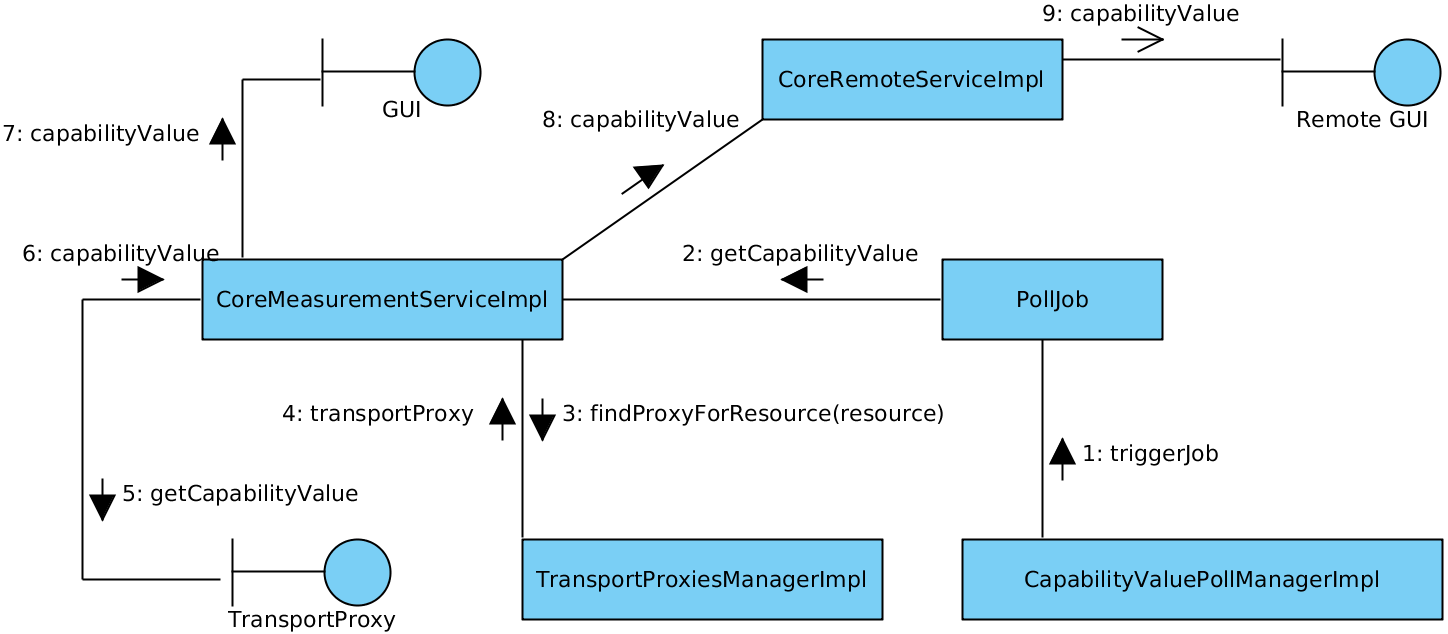
\includegraphics[width=1\textwidth]{comm_mh_new_cap_val}
  \caption{Monitoring Hub Communication diagram - new capability value notification}
  \label{fig:comm_new_cap_val}
\end{figure}

\pagebreak